% (c) 2020 Stefan Antonowicz
% Based off of tex found at https://github.com/ludus-leonis/nipajin
% This file is released under Creative Commons Attribution-NonCommercial-ShareAlike 4.0 International License.
% Please do not apply other licenses one-way.

\renewcommand{\yggSkillsSaves}{%
  \mychapter{Skills and Saves}{skills-and-saves}
}

\renewcommand{\yggSkillsSavesText}{%
  \mysection{Skills}{skills}

  \example {
    \RO: \STATIC \PLUS \mybold{d20} \PLUS Bonus \PLUS Modifiers 
  }

  Skills rolls are \RO tries to see if something is possible and achievable.  The Arbiter should only call for a Skills roll when the difference between success and failure would be interesting, or when a skill that's not interesting enough to describe still shouldn't be an automatic success.

  Each Skill has a level attached to it to describe how rad you are:

  \mytable{X c c c}{
    \thead{Skill} & \thead{\STATIC} & \thead{Bonus} & \thead{Successes} \\
  }{
      Untrained & d4 & +0 & 0 \\
      Trained  & d8 & +1 & 10 \\
      Skilled & d12 & +2 & 25 \\
      Master  & d20 & +3 & 50 \\
      Artist  & d24 & +4 & 100 \\
  }




  \mysubsection{Successes}{skills-achievements}

  Whenever you succeed at using a Skill, put a checkmark or number next to it.  When you hit the number of successes shown in the chart above, your Skill goes up a level (for example, if you were to succeed 10 times when using your Salt skill, your skill would go from "Untrained" to "Trained").  Skills that start at Trained level because of your Trope have 10 successes already attached to them.

  Just remember that it is the Arbiter who decides whether or not a Skill check is necessary or can be attempted - when the difference between success and failure would be interesting, or when a skill that's not interesting enough to describe still shouldn't be an automatic success.  You can certainly suggest it, but the ultimate decision rests on the Arbiter.


   \mysubsection{Books}{skills-books}

   You may stumble across certain books that contain instructions, histories, theories, etc. that can assist you in making a Skill check.  If used as a reference, these books can provide a bonus between +1 (for a primer on Tea Ceremonies, say) to +3 (the definitive multi-volume history of Elfland) where appropriate. 

   Other books might allow you to learn a Skill during a Vacation.  In this case, the book can't bring your level higher than "Trained".


  \mysubsection{Helping Out}{skills-helping-out}

  Maybe the runes are a little bit harder to decipher than you thought; maybe it's really important you not get lost in the woods right now.  If you want to hedge your bets a little, you can ask for help from \mybold{one} other adventurer.  The helper adds their Bonus to your roll (this is in addition to any other modifiers).  Again, only \mybold{one} adventurer can help you out, unless they are a Pooka (in which case, they don't count against your one person).

  If you succeed, you get the credit for the success.  If the other adventurer has a lower Bonus than you do, they also get credit for the success.

  \example {
      Tony "Two Touch" Tomlinnson is Skilled (d12,+2) at Bushcraft, but he's a little worried about getting lost. He asks for Kurt Eberwulf's help - Kurt is also Skilled, so Tony rolls a d20 + d12+2 (for being Skilled at Bushcraft) + 2 (for Kurt's help).  He's able to \RO (gets a 25) and he gets credit for the success.  If Kurt had been only Trained (+d8,+1) in Bushcraft, he would have received credit for the success also, but since he and Tony are the same level he doesn't learn anything new.
  }

  The person helping has to describe to the Arbiter how they're helping you; if it doesn't sound feasible, the bonus doesn't get applied.


  \mysubsection{Possibility}{skills-possibility}

  For Skills, the \RO roll doesn't just determine success, but \myital{whether or not something is even possible}.  

  If you fail at interpreting those twisting eldritch runes (Lore), it means that it's simply not possible in these conditions.  Maybe it's your fault, maybe it isn't.  The runes can't be made out, or this is only a fragment, or whatever.  Who knows.  It's just not possible - you tried, failed, and now you know.

  If you have a sailor adventuring with you whose Salt is Skilled (d12,+2), they're going to have a better chance of success.  But if someone fails a Salt roll before the sailor had a chance to try, then they fucked it all up (they didn't shiver the timbers or hoist the mainsail or forgot about high tide or what-have-you).  They should have waited for the professional to give it a shot.  This might be a permanent or temporary condition at the Arbiter's discretion.

  After the first adventuerer succeeds, everyone else is able to follow along behind them.  Additional skill checks won't have any effect on whether something is possible or not.  If adventurer 1 succeeds, it's possible - adventurer 2 failing doesn't suddenly make it impossible.  If further Skills rolls are necessary, everyone who follows after the first adventurer adds that adventurer's Bonus to their Skills roll.

    \begin{center}
  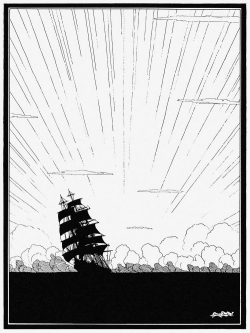
\includegraphics[scale=.5]{Ship}
  \end{center}
 
  \cbreak

  \mysubsection{The Core Skills}{skills-list}

  There are 7 Core Skills.  You being Untrained in every Skill, though your Trope or Species might bump these up to Trained during character creation:

  \mylist {
    \item \myanchor{\mybold{Bushcraft}}{skill-bushcraft} tracking, hunting, camping, finding water, survival, making fires, ranger shit
    \item \myanchor{\mybold{Eyeball}}{skill-eyeball} estimate something's value or weight; size somebody up; judge distance, quality, etc 
    \item \myanchor{\mybold{Listen}}{skill-listen}  listen at doors, remember something the Arbiter told you that you've forgotten
    \item \myanchor{\mybold{Lore}}{skill-lore}  general ancient knowledge - esoteric religions, what the weird writing says, history of this magic item, whether or not something is a component 
    \item \myanchor{\mybold{Math}}{skill-math} architecture, sloping rooms, construction, where a secret door might be 
    \item \myanchor{\mybold{Salt}}{skill-salt} swimming, sailing boats, having sea-legs, fishing, navigating by the stars, tying knots
    \item \myanchor{\mybold{Travel}}{skill-travel} estimating food and water for a convoy; riding horses and camels; mountain climbing 
  }




  \mysubsection{Other Skills}{skills-other}

    The 7 Core Skills are the basics skills that everyone gets.  You can add another skill to your character sheet based on your character history (you were a Haberdasher in Lankhmar and now you have Skill: Tailoring), and you may also find additional skills by reading books, apprenticeships, etc (for example, you might find a book on teacups or something and you spend a Vacation reading it and now you have the Skill: Tea Ceremony).

    Here are a few other Skills mentioned in these rules.

  \mylist {
    \item \myanchor{\mybold{Veins Lore:}}{skill-veins-lore}   Any time you encounter something in the \mylink{Veins}{murk-veins-of-the-earth} you might not understand, you can try this roll.  Some examples:  remembering what kind of gift is appropriate to give to an Ambassodile, what that smell is in the darkness, figuring out what kind of architect this Janeen is, etc.  If you are a Murk and were a slave of the culture you're rolling against, you get a +2 bonus.
    
    \item \myanchor{\mybold{Tinkering:}}{skill-tinkering}   The skill of fixing, understanding and manipulating small devices and tools.  A shittier, non-magic version of Knave Whispers, most often  used by scavengers to disarm small mechanical traps or their triggers, picking simple locks, and to trying to repair broken stuff.  If you fail your Tinker roll the worst possible event happens i.e. the trap explodes for maximum damage, the weapon you're "fixing" is destroyed beyond repair, the improvised lockpick breaks and now no-one can pick the lock, etc.  You can use Tinker during a Bivouac to try to repair a \UD of Armor, but if you fail you make it 1 \UD \mybold{worse}

    \item \myanchor{\mybold{Linguistics:}}{skill-linguistics}   Any time you encounter a written language you can't read, you can try this roll.  If you succeed the Arbiter can give you a general idea of what the text says, but not specifics. You can't use this skill to read magical writing (scrolls, spell books, etc)

  }

  \mysection{Saves}{saves}

  \example {
    \RO: \STATIC \PLUS \mybold{d20} \PLUS Bonus \PLUS Modifiers 
  }

  You missed the poison needle in the chest, got too close to the dragon's flame, didn't kill the swamp hag before she pointed her magic wand at you and caused snakes to shoot out and try to bite you on your stupid face.

  Like Skills, each Save has a level attached to it to describe how rad you are:


    \mytable{X c c}{
    \thead{Skill/Save} & \thead{\STATIC} & \thead{Bonus} \\
  }{
      Defenseless & d4 & +0 \\
      Preserved  & d8 & +1 \\
      Protected & d12 & +2 \\
      Strong & d20 & +3 \\
      Unbeatable & d24 & +4 \\
  }


 \cbreak

    \begin{center}
  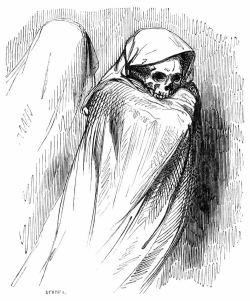
\includegraphics[scale=.75]{CloakDeath}
  \end{center}

  There are 3 types of Saves in ToY:

  \mylist {
    \item \myanchor{\mybold{Hexes}}{save-hexes}  - this includes certain spells and magical effects. If a spell description says "Save for half damage", this is the Save you roll.
    \item \myanchor{\mybold{Toxins}}{save-toxins}  - various and sundry poisons and diseases.  If a poison or disease description says "Save or suffer d100 damage", this is the Save you roll.
    \item \myanchor{\mybold{Doom}}{save-doom}  - includes dragon's breath, the gaze of a medusa, or things that might kill you outright.  If a Monster's description says something like "Save or die", this is the Save you roll.
  }

  At character creation, pick one Save - you are Sensitive (d8,+1) with that Save.  All the other Saves are Defenseless.

} %end
